\section {Cronograma de actividades}
\begin{figure}[H]
En primer semestre se recolectará información de forma aislada así como integrada con aplicaciones afines al proyecto.

Durante segundo semestre se construirán los modelos para obtener de la base de datos.

En tercer semestre se obtendrá el conjunto de palabras para extender la búsqueda y estimar modelos de regresión, y se realizará una búsqueda correlacionada complementaria.

En cuarto semestre se obtendrán nuevos modelos de regresión lineal utilizando los datos de la búsqueda y se realizarán pruebas de hipótesis del modelo anterior para obtener mejores estimadores. Se construirán elementos gráficos usando distribuciones y rectas de regresión lineal y se comunicarán los resultados.\\
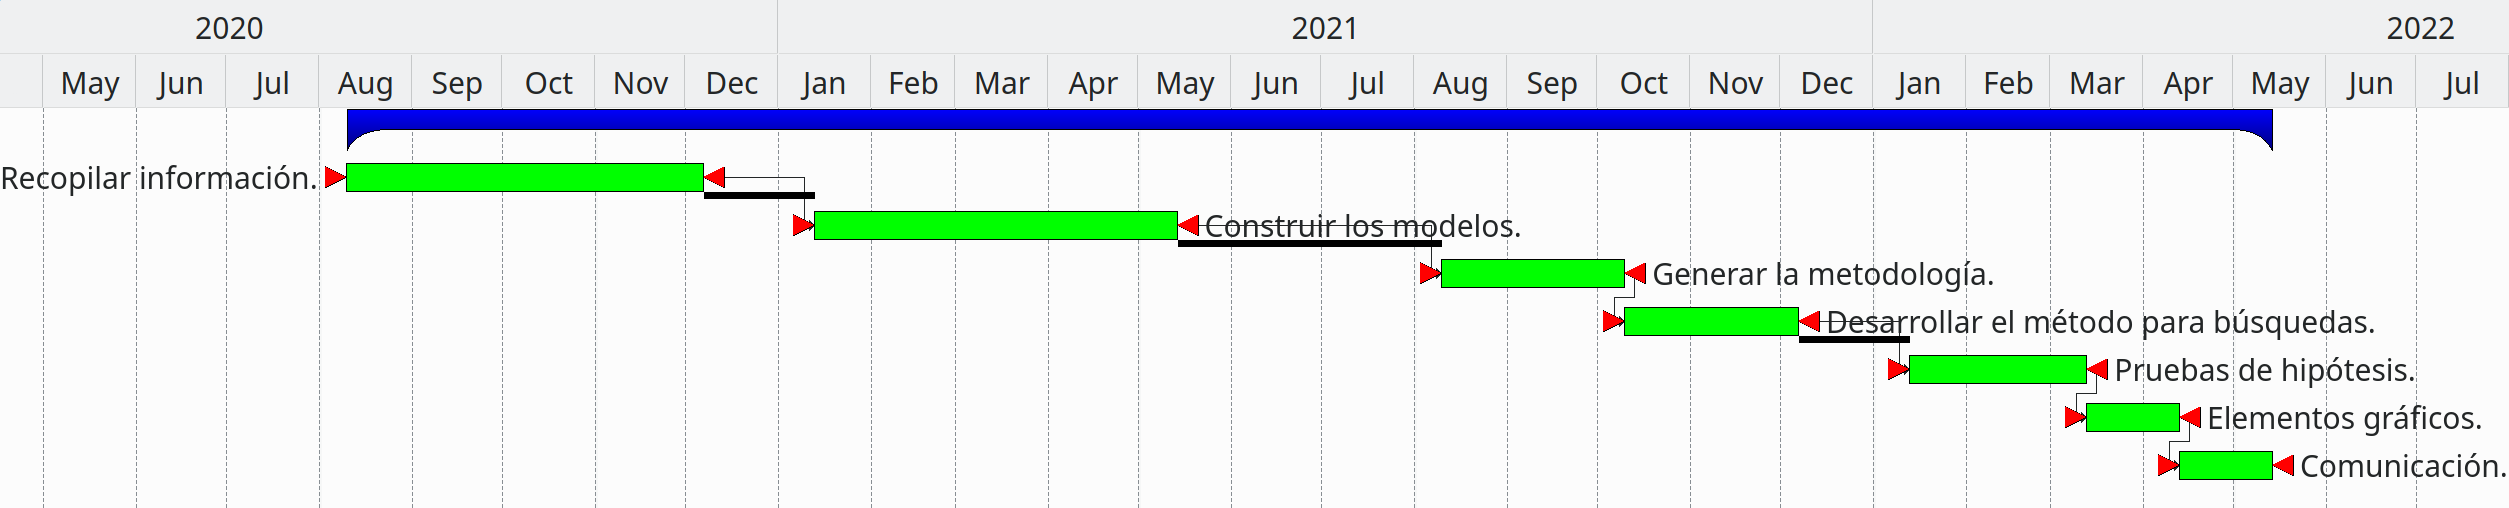
\includegraphics[width=1\linewidth]{gantt.png}\end{figure}